\documentclass[a4j]{jarticle}

\usepackage[dvipdfmx]{graphicx}
\usepackage{url}
\usepackage{here}
%\usepackage{listings}
\usepackage{amsmath,amssymb}
\usepackage[dvipdfmx]{color}

\setlength{\headsep}{-5mm}
\setlength{\oddsidemargin}{0mm}
\setlength{\textwidth}{165mm}
\setlength{\textheight}{230mm}
\setlength{\footskip}{20mm}

%% 本文
\begin{document}
\section{フロー図}

\begin{figure}[H]
\begin{center}
\resizebox{16.5cm}{!}{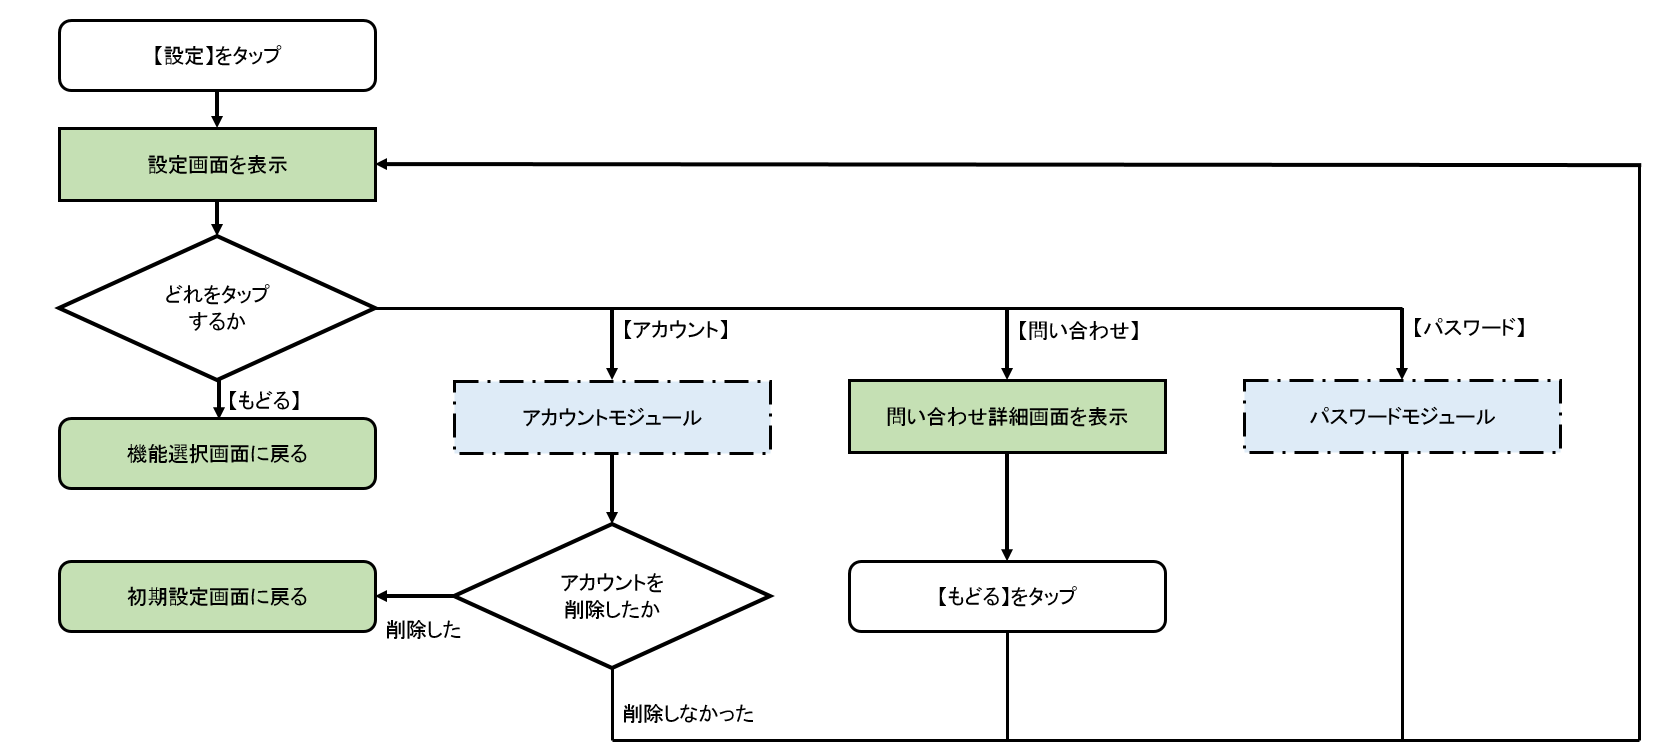
\includegraphics{設定_全体.png}}
\caption{設定機能全体}
\label{allgrow}
\end{center}
\end{figure}

\begin{figure}[H]
\begin{center}
\resizebox{16.5cm}{!}{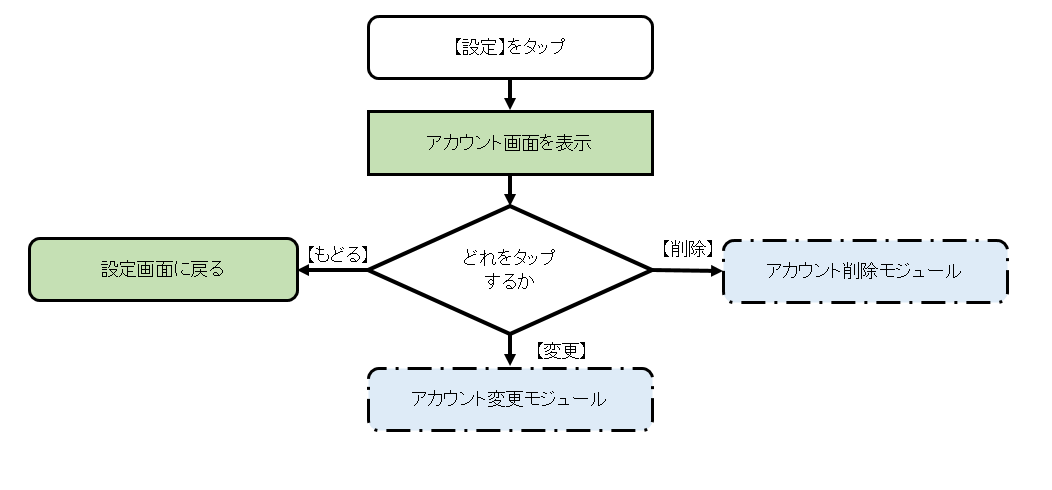
\includegraphics{設定_アカウント.png}}
\caption{アカウントモジュール}
\label{deletemoju}
\end{center}
\end{figure}

\begin{figure}[H]
\begin{center}
\resizebox{16.5cm}{!}{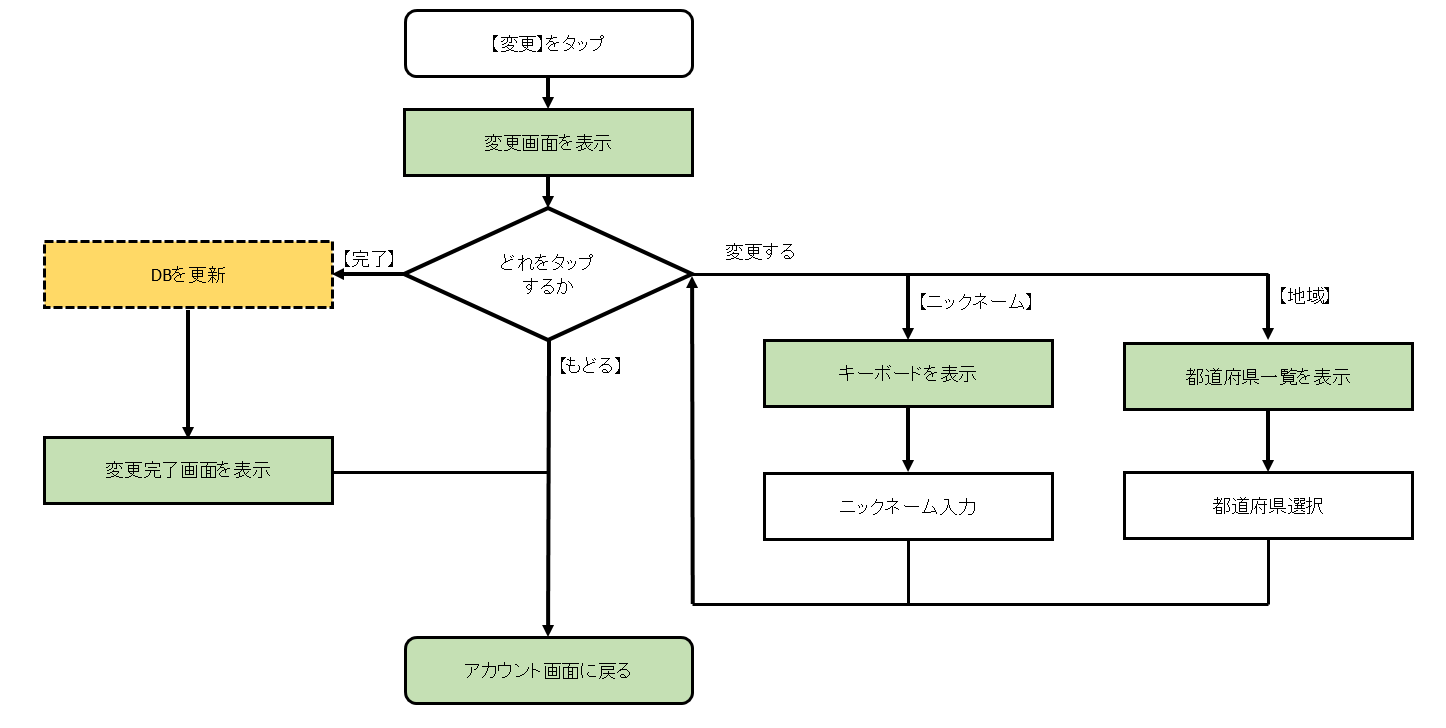
\includegraphics{設定_変更.png}}
\caption{変更モジュール}
\label{alubammoju}
\end{center}
\end{figure}

\begin{figure}[H]
\begin{center}
\resizebox{16.5cm}{!}{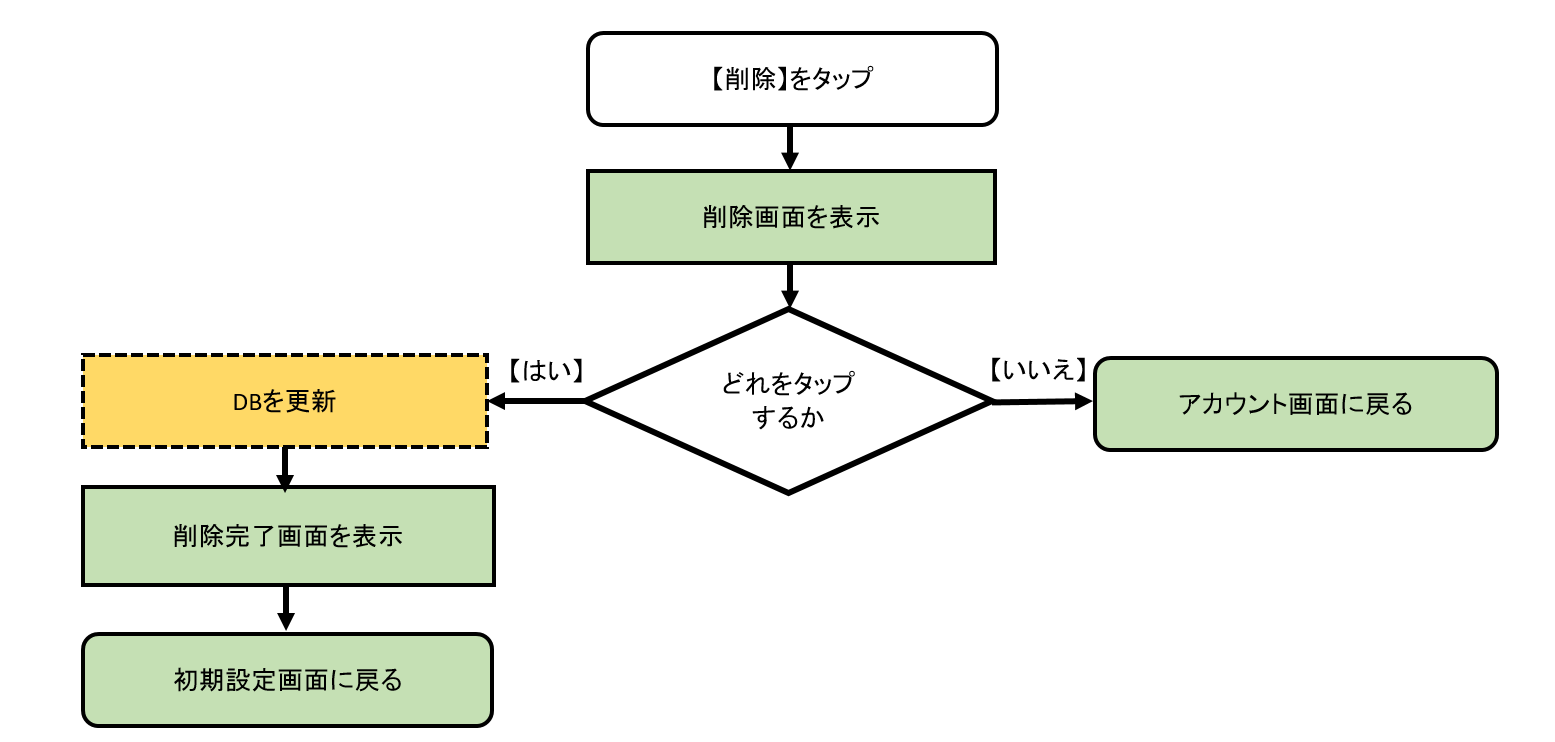
\includegraphics{設定_削除.png}}
\caption{削除モジュール}
\label{cameramoju}
\end{center}
\end{figure}

\begin{figure}[H]
\begin{center}
\resizebox{16.5cm}{!}{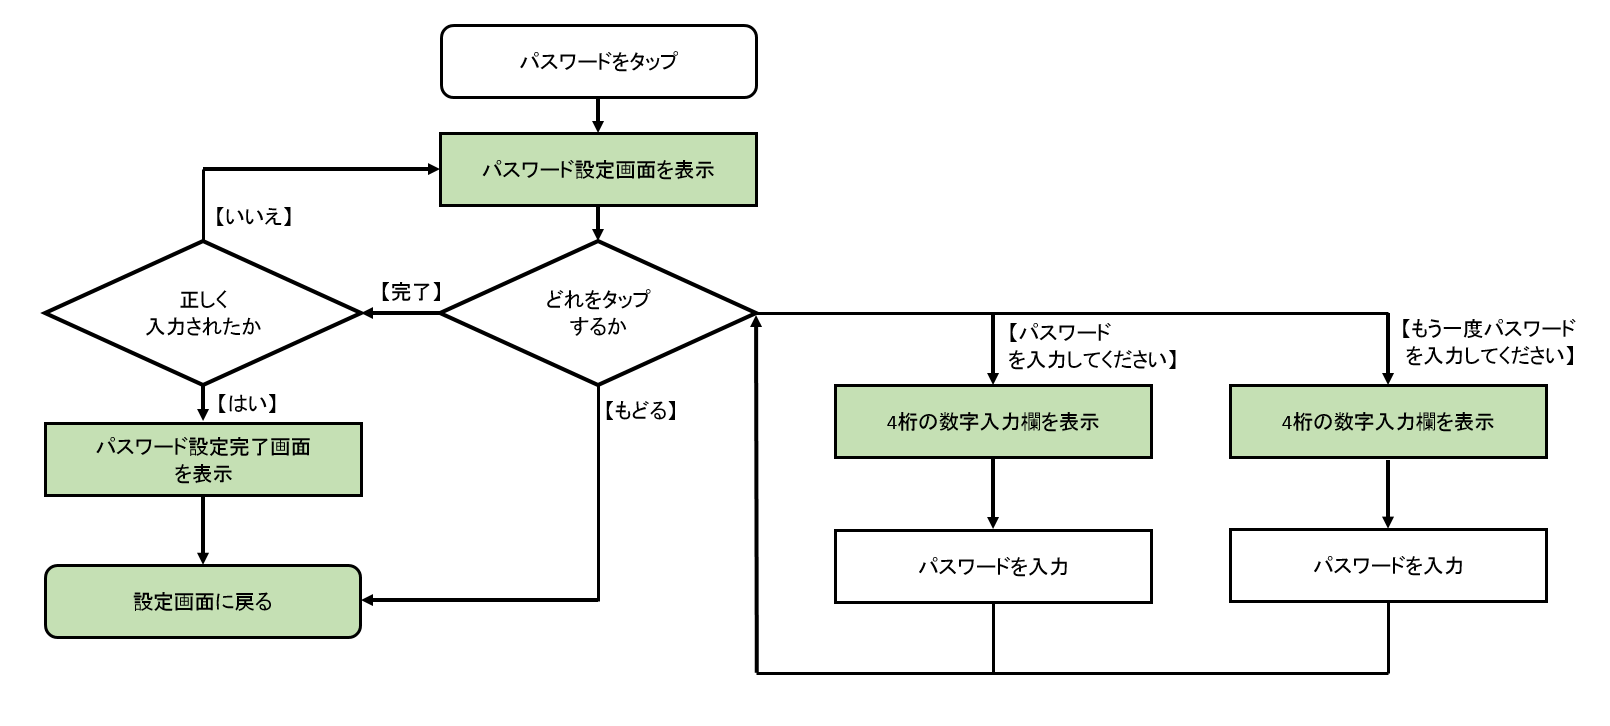
\includegraphics{設定_パスワード.png}}
\caption{パスワードモジュール}
\label{comentmoju}
\end{center}
\end{figure}

\section{モジュール}
各モジュールの説明を行う

\subsection{設定機能全体}
\subsubsection*{概要}本システムはSNS機能を利用する際に必要なアカウントの登録を行うことができます。また。アカウントの変更・削除も行うことができます。他に、こどもがゲーム機能を使用する際に他の機能や本システム以外のシステムを触らないようにパスワードの設定も行います。
機能としては、アカウントモジュール、変更モジュール、削除モジュール、パスワードモジュールがあります。

\subsubsection*{処理フロー}
\begin{itemize}
\item 【アカウント】をタップすることでアカウントモジュールを呼び出します。その後アカウントが削除されたかどうかで設定画面か初期設定画面に遷移します。

\item 【問い合わせ】ボタンをタップすることで問い合わせ詳細画面を表示します。その後【もどる】ボタンをタップすることで設定画面に戻ります。

\item 【パスワード】をタップすることでパスワードモジュールを呼び出します。

\item 【もどる】をタップすることで機能設定画面に戻ります。
\end{itemize}

\subsection{アカウントモジュール}
\subsubsection*{概要}SNSを利用する際のアカウントの登録・変更・削除を行う機能です。

\subsubsection*{処理フロー}
\begin{itemize}
\item 【変更】をタップすることで変更モジュールを呼び出します。
\item 【削除】をタップすることで削除モジュールを呼び出します。
\item 【もどる】をタップすることで設定画面に戻ります。
\end{itemize}

\subsection{変更モジュール}
\subsubsection*{概要}アカウントの変更を行う機能です。

\subsubsection*{処理フロー}
\begin{itemize}
\item 【ニックネーム】をタップすることでニックネームの変更を行います。
\item 【地域】をタップすることで地域の変更を行います。
\item 【完了】をタップした場合【ニックネーム】と【地域】の設定が正しく行われていればDBを更新しアカウントの変更を行います。
\item 【もどる】ボタンをタップすることでアカウント画面に戻ります。
\end{itemize}

\subsection{削除モジュール}
\subsubsection*{概要}アカウントの削除を行うモジュールです。

\subsubsection*{処理フロー}
\begin{itemize}
\item 【はい】をタップすることでDBを更新しアカウントの削除を行います。その後削除完了画面を表示し初期設定画面に戻ります。
\item 【いいえ】をタップすることでアカウント画面に戻ります。
\end{itemize}

\subsection{パスワードモジュール}
\subsubsection*{概要}こどもがゲーム機能を利用する際に他の機能や他のシステムを利用できないようにパスワードを設定する機能です。

\subsubsection*{処理フロー}
\begin{itemize}
\item 【パスワードを入力してください】をタップし4桁の数字を入力することでパスワードの設定を行います。
\item【もう一度パスワードを入力してください】をタップし4桁のパスワードを入力することでパスワードの確認を行います。
\item 【完了】をタップした場合パスワードが正しく入力されていればパスワード設定画面完了画面を表示し設定画面に戻ります。正しく入力されていなければパスワード設定画面に戻ります。
\item 【もどる】をタップすることで設定画面に戻ります。

\end{document}